\documentclass[12pt, a4paper, oneside, openright]{thesis}

\usepackage[T1]{fontenc}
\usepackage[utf8]{inputenc}
\usepackage{lmodern}

\usepackage[english, spanish, catalan]{babel}
\usepackage[catalan]{translator}

\usepackage[style=bibstyles/myieee,backref=true,backend=biber]{biblatex}
\addbibresource{cap2/bib/biblio.bib}
\addbibresource{cap3/bib/biblio.bib}
\addbibresource{cap4/bib/biblio.bib}
\addbibresource{cap5/bib/biblio.bib}
\addbibresource{app/biblio.bib}


\usepackage[toc, acronyms]{glossaries}

\makeglossaries
\loadglsentries{abbrevs}

% comments
\usepackage{verbatim}

\usepackage{blindtext}
\usepackage{lipsum}

\usepackage{listing}
\usepackage[section, outputdir=build]{minted}

\usepackage{tcolorbox}
\tcbuselibrary{minted,skins}

\newtcblisting{pythoncode}{
	listing engine=minted,
	colback=bg,
	colframe=black!70,
	listing only,
	minted style=monokai,
	minted language=python,
	minted options={linenos=true,texcl=true},
	left=1mm,
}
\definecolor{bg}{HTML}{282828}

%%%%%%%%%%%%%%%%%%%%%%%%%%%%%%%%%%%%%%%%%%%%%%%%%%%%%%%%%%%%%%%%%%%%%%%%%%%%%%%
% AMS MATH %%%%%%%%%%%%%%%%%%%%%%%%%%%%%%%%%%%%%%%%%%%%%%%%%%%%%%%%%%%%%%%%%%%%
%%%%%%%%%%%%%%%%%%%%%%%%%%%%%%%%%%%%%%%%%%%%%%%%%%%%%%%%%%%%%%%%%%%%%%%%%%%%%%%
\usepackage{amsmath}        % loads amstext, amsbsy, amsopn but not amssymb
                            % equation stuff (eqref, subequations, equation, align, gather, flalign, multline, alignat, split...)
% \usepackage{amsfonts}     % may be redundant with amsmath
% \usepackage{amssymb}      % may be redundant with amsmath
% \numberwithin{equation}{section}  % reset equation counters at start of each "section" and prefix numbers by section number
% \numberwithin{figure}{section}    % reset figure   counters at start of each "section" and prefix numbers by section number

\usepackage{tikz}
\usetikzlibrary{matrix,chains,positioning,decorations.pathreplacing,arrows,intersections}

\usepackage{pgfplots}
\usepgfplotslibrary{fillbetween}

\usepackage{graphicx}
\graphicspath{ 
	{cap5/img/}
	{cap3/img/}
}

\usepackage{neuralnetwork}

\usepackage{caption}
\usepackage{subcaption}

\usepackage{float}

\usepackage{algpseudocode, algorithm, algorithmicx}

\usepackage[
  pdfauthor={Stepan Klymonchuk},
  pdftitle={Intel.ligència Artificial},
  colorlinks=true,
  linktocpage=false,
  hyperindex=true,
  linkcolor=.,
  urlcolor=blue,
  citecolor=green,
  anchorcolor=red,
  filecolor=magenta,
  bookmarks=true,
  hypertexnames=true,
  pdfencoding=auto
]{hyperref}

\usepackage{bookmark}
\usepackage[all]{hypcap}

\usepackage{cleveref}

% red references
\let\oldcref\cref
\renewcommand{\cref}[1]{\hypersetup{linkcolor=red}\oldcref{#1}\hypersetup{linkcolor=.}}%<<<changed

% red page references
\let\oldprintbibliography\printbibliography
\renewcommand{\printbibliography}[1][]{\hypersetup{linkcolor=red}\oldprintbibliography[#1]\hypersetup{linkcolor=.}}%<<<changed

\usepackage[toc,page,title,titletoc]{appendix}

\usepackage[a4paper,margin=2.54cm]{geometry}

% bold vectors
\let\oldhat\hat
\renewcommand{\vec}[1]{\mathbf{#1}}
\renewcommand{\hat}[1]{\oldhat{\mathbf{#1}}}

\setlength{\parindent}{0em}
\setlength{\parskip}{1em}
\renewcommand{\baselinestretch}{1.15}

\setbox0=\hbox{\ttfamily}

\renewcommand{\appendixtocname}{Apèndixs}
\renewcommand{\appendixpagename}{Apèndixs}
\renewcommand{\appendixname}{Apèndix}

\makeatletter
\let\oriAlph\Alph
\let\orialph\alph
\renewcommand{\@resets@pp}{
  \par
  \@ppsavesec
  \stepcounter{@pps}
  \setcounter{section}{0}
  \if@chapter@pp
    \setcounter{chapter}{0}
    \renewcommand\@chapapp{\appendixname}
    \renewcommand\thechapter{\@Alph\c@chapter}
  \else
    \setcounter{subsection}{0}
    \renewcommand\thesection{\@Alph\c@section}
  \fi
  \if@pphyper
    \if@chapter@pp
      \renewcommand{\theHchapter}{\theH@pps.\oriAlph{chapter}}
    \else
      \renewcommand{\theHsection}{\theH@pps.\oriAlph{section}}
    \fi
    \def\Hy@chapapp{appendix}
  \fi
  \restoreapp
}
\makeatother

\begin{document}

\frontmatter

\begin{titlepage}
	\begin{center}
		\vspace*{1cm}
		
		\Large
		Treball de Recerca
		
		\vspace{1.5cm}

		\Huge
		\textbf{Intel·ligència Artificial}

		\vspace{1cm}

		\LARGE
		Aprenentatge Automàtic i Xarxes Neuronals
		aplicats als entorns virtuals i reals

		\vspace{1.5cm}

		\textbf{Stepan Klymonchuk}

		\vfill
		\Large
		Tutor: Raül Bercet\\
		Institut Narcís Oller\\
		\today
	\end{center}
\end{titlepage}
\newpage

\setcounter{page}{2}

\begin{center}
	\vspace*{\fill}
	\textit{A la meva família}
	\vspace*{\fill}
\end{center}

\newpage

%\addtocontents{toc}{\vspace{1em}}
%\chapter*{Agraïments}
\setcounter{chapter}{-6}
\addcontentsline{toc}{chapter}{Agraïments}

Agraïments

%\newpage

\begin{otherlanguage}{english}

	\chapter*{Abstract}
	\setcounter{chapter}{-4}
	\addcontentsline{toc}{chapter}{Abstract}
	
	In computer science, artificial intelligence (AI) is an intelligence presented by machines, unlike the natural intelligence shown by humans and animals. This field of computing is devoted to the development of algorithms that can be implemented on machines so that they make decisions and, therefore, provide them with a certain intelligence to perform cognitive functions that imitate human beings, such as learning and solving problems. In recent years the field of artificial intelligence has evolved a great deal, to such an extent that today many companies have developed intelligent systems capable of reaching points that no one would have thought before. Most of the AI examples that currently exist, from computers that play chess to voice recognition and autonomous vehicles, largely depend on deep learning and the processing of natural language. By using these technologies, computers can be trained to perform certain tasks by processing large amounts of data and recognizing patterns. In this work, an introduction will be made to the world of neuronal networks and deep learning to try to recognize and classify manuscript digits with a high percentage of success, testing different architectures of neural networks and varying their parameters.
	
\end{otherlanguage}

\newpage

\begin{otherlanguage}{catalan}

	\chapter*{Resum}
	\setcounter{chapter}{-3}
	\addcontentsline{toc}{chapter}{Resum}

	En ciències de la computació, la intel·ligència artificial (IA) és una intel·ligència que presenten les màquines, a diferència de la intel·ligència natural que mostren els humans i els animals. Aquest camp d’informàtica es dedica al desenvolupament d’algoritmes que es puguin implementar en màquines perquè aquestes prenguin decisions i, per tant, dotar-les de certa intel·ligència per realitzar funcions cognitives que imiten a les humanes, com ara \textit{aprendre} i \textit{resoldre problemes}. En els últims anys el camp la intel·ligència artificial ha evolucionat molt, fins a tal punt que avui en dia moltes companyies han desenvolupat sistemes intel·ligents capaços d'arribar a punts que anys enrere ningú s'hauria pensat. La majoria dels exemples de la IA que existeixen actualment, des dels ordinadors que juguen als escacs fins al reconeixement de veu i els vehicles autònoms, depenen en gran manera de l’aprenentatge profund i del processament del llenguatge natural. Utilitzant aquestes tecnologies, els ordinadors poden ser entrenats per realitzar determinades tasques processant grans quantitats de dades i reconeixent patrons. En aquest treball es realitzarà una introducció al món de les xarxes neuronals i l'aprenentatge profund per intentar reconèixer i classificar dígits manuscrits amb un alt percentatge d'encert, provant diferents arquitectures de xarxes neuronals i variant els seus paràmetres.

\end{otherlanguage}

\newpage

\begin{otherlanguage}{spanish}

	\chapter*{Resumen}
	\setcounter{chapter}{-2}
	\addcontentsline{toc}{chapter}{Resumen}

	En ciencias de la computación, la inteligencia artificial (IA) es una inteligencia que presentan las máquinas, a diferencia de la inteligencia natural que muestran los humanos y los animales. Este campo de informática se dedica al desarrollo de algoritmos que se puedan implementar en máquinas para que estas tomen decisiones y, por tanto, dotarlas de cierta inteligencia para realizar funciones cognitivas que imitan a las humanas, tales como aprender y resolver problemas. En los últimos años el campo la inteligencia artificial ha evolucionado mucho, hasta tal punto que hoy en día muchas compañías han desarrollado sistemas inteligentes capaces de llegar a puntos que años atrás nadie habría pensado. La mayoría de los ejemplos de la IA que existen actualmente, desde los ordenadores que juegan al ajedrez hasta el reconocimiento de voz y los vehículos autónomos, dependen en gran medida del aprendizaje profundo y del procesamiento del lenguaje natural. Utilizando estas tecnologías, los ordenadores pueden ser entrenados para realizar determinadas tareas procesando grandes cantidades de datos y reconociendo patrones. En este trabajo se realizará una introducción al mundo de las redes neuronales y el aprendizaje profundo para intentar reconocer y clasificar dígitos manuscritos con un alto porcentaje de acierto, probando diferentes arquitecturas de redes neuronales y variando sus parámetros.

\end{otherlanguage}

\addtocontents{toc}{\vspace{1em}}
\newpage

\begin{flushright}
	\vspace*{\fill}
	\textit{La gent que no es creu que les matemàtiques són senzilles,
		és només que no s'ha adonat de com és de complicada la vida.}
	
	J. L. Von Neumann
	\vspace*{\fill}
\end{flushright}

\newpage

%\include{intro/index}
%\newpage

\chapter*{\contentsname}
\setcounter{chapter}{-1}
\addcontentsline{toc}{chapter}{\contentsname}
\tableofcontents*

\chapter*{\listfigurename}
\setcounter{chapter}{0}
\addcontentsline{toc}{chapter}{\listfigurename}
\listoffigures*

%\chapter*{\listtablename}
%\setcounter{chapter}{0}
%\addcontentsline{toc}{chapter}{\listtablename}
%\listoftables*

\renewcommand\listingscaption{Listing}
\renewcommand{\listlistingname}{Índex de listings}

\listoflistings
\addcontentsline{toc}{chapter}{\listlistingname}

\renewcommand*{\acronymname}{Abreviacions}
\printglossary[type=\acronymtype, toctitle=\acronymname]

\addtocontents{toc}{\vspace{1em}}

\newpage

\mainmatter

\begin{refsection}

	\chapter{Introducció}

	\section{Motivació}

	A l'hora de triar el tema del treball de recerca vaig pensar que m'agradaria fer-lo de programació, però no només duna manera abstracta, sinó en relació amb alguna aplicació concreta que tingués a veure amb els meus interessos. Un dia vaig descobrir què eren les xarxes neuronals i la intel·ligència artificial. D'una banda, em vaig adonar que existeixen molts mites i molta desinformació sobre el tema de la IA: la intel·ligència artificial substituirà tots els llocs de treball, superarà la intel·ligència humana o conduirà a l'esclavitud de la nostra raça per part dels éssers robòtics superiors, com es descriu en diverses pel·lícules i històries de ciència-ficció.

	De l'altra banda, em va sorprendre la quantitat d'aplicacions que té la IA actualment  (concretament l'aprenentatge automàtic i les xarxes neuronals) i la seva important presència en el nostre dia a dia. D'aquesta manera, després d'haver fet recerca per informar-me del tema, sem van acudir aquestes preguntes:

	\begin{itemize}
		\item Poden els ordinadors aprendre de l'experiència com nosaltres, humans?
		\item Què són les xarxes neuronals i perquè són tan útils?
		\item Com ho fan les xarxes neuronals per reconèixer imatges?
		\item Quins altres mètodes d'aprenentatge automàtic hi ha a part de les xarxes neuronals?
	\end{itemize}

	A partir d'aquestes preguntes vaig decidir fer un treball relacionat amb la intel·ligència artificial.

	El fet d'haver triat aquest tema també està motivat pel meu interès per les matemàtiques perquè estan relacionades amb la programació. A grans trets el treball consisteix, per una banda, en entendre què és la IA, l'aprenentatge automàtic i les xarxes neuronals, com funcionen, quines són les seves aplicacions, etc. i, per l'altra, en dissenyar i programar models de xarxes neuronals i aplicar-les als entorns reals i virtuals per resoldre problemes concrets.

	\section{Objectius}

	Concretament els objectius d'aquest treball són:

	\begin{itemize}

		\item Investigar en àrees d'IA, informàtica, i programació per aprendre conceptes que poden ser aplicats en diferents àrees com l'anàlisi d'imatges o presa de decisions.

		\item Explicar el funcionament de diferents mètodes d'aprenentatge automàtic (centrant-se principalment en les xarxes neuronals).

		\item Demostrar que els sistemes d'aprenentatge automàtic són útils i aplicables.

		\item Comprendre els conceptes, el funcionament i l'abast de les xarxes neuronals i mostrar el procés de disseny i implementació de xarxes neuronals amb TensorFlow i Keras per aconseguir objectius específics.

	\end{itemize}

	En el camp de visió artificial (Reconeixement d'imatges):

	\begin{itemize}

		\item Dissenyar i implementar un model predictiu eficaç en la classificació de dígits escrits a mà utilitzant el conjunt de dades MNIST.

		\item Analitzar el funcionament i el rendiment de diferents arquitectures de xarxes neuronals.

	\end{itemize}

	\begin{comment}

	Videojocs (presa de decisions):

	\begin{itemize}

		\item Adaptar la metodologia d'aprenentatge per reforçament d'AlphaZero de Google DeepMind per a jocs com connecta 4 o gomoku.

		\item Analitzar el funcionament dels algoritmes emprats en AlphaZero (arbre de cerca de Monte Carlo, MCTS).

		\item Entrenar un agent de Deep Q Learning (DQN) per realitzar tasques de OpenAI Gym (videojocs i simulacions diferents) i analizar el seu rendiment.
	\end{itemize}

	\end{comment}

	\addtocontents{toc}{\vspace{1em}}
	\printbibliography[heading=subbibintoc]

\end{refsection}

\newpage

\begin{refsection}

	\chapter{Intel·ligència artificial}
	\label{chap:AI}

	\section{Història}
	
	Tot i que els primers referents històrics es remunten als anys 30 amb Alan Turing, considerat el pare de la intel·ligència artificial, es considera que el punt de partida és l'any 1950, precisament, quan Turing publica un article amb el títol \textit{Computing machinery and intelligence} a la revista Mind, on es va plantejar la pregunta: poden pensar les màquines? I proposa un mètode per determinar si una màquina pot pensar. Els fonaments teòrics de la IA es troben en l'experiment que es proposa en aquest article i que va passar a anomenar-se test de Turing. Mitjançant la superació d'aquest test per una màquina, és possible que la màquina pugui passar per un ésser humà. El test manté la seva vigència en l'actualitat i és el motiu d'estudis i investigacions contínues.\supercite{Breuhist}
	
	No obstant això, nombrosos investigadors i historiadors consideren que el punt de partida de la intel·ligència artificial moderna va ser l'any 1956, quan els pares de la intel·ligència artificial moderna, John McCarty, Marvin Misky i Claude Shannon van definir formalment el terme durant la conferència de Darmouth com \textit{la ciència i l'enginy de fer màquines intel·ligents, especialment programes de càlcul intel·ligent}.\supercite{LiveScience}
	
	El supercomputador Deep Blue d'IBM va guanyar el 1997 al campió mundial d'escacs Gari Kaspàrov, després d'un fracàs previ en 1996 on va guanyar Kaspàrov. L'any 1997 és considerat per alguns historiadors de la IA com el punt d'inflexió on va començar a sentir-se de la intel·ligència artificial fora dels àmbits acadèmics i de recerca.\supercite{Breuhist}.
	
	Al febrer de 2011, el supercomputador Watson d'IBM, el model de computador cognitiu, com l'anomena el seu creador IBM, guanya al concurs televisiu dels Estats Units \textit{Jeopardy!}, en el qual es realitzen preguntes i qüestions diferents de tota mena, cultura i coneixement, als dos millors concursants del programa, Brad Ruttler i Ken Jennings.\supercite{aiwiki}
	
	Una altre fet important va ser la presentació d'Apple de l'assistent virtual Siri integrat al telèfon mòbil iPhone 4S a l'any 2011 i on van començar les primeres experiències d'aprenentatge automàtic i els primers indicis d'aprenentatge profund.\supercite{NationalGeographic}
	
	L'any 2012 és considerat com l'any clau de la segona generació d'intel·ligència artificial, amb el llançament d'assistents virtuals recolzats en IA amb algoritmes d'aprenentatge profund. Al juny de 2012 Google va presentar el seu assistent virtual, Google Now, i a l'abril de 2014 Microsoft va presentar el seu propi assistent virtual, Cortana.\supercite{aiwiki}
	
	El 9 de març de 2016, el programari d'intel·ligència artificial Alpha Go de Google DeepMind es va enfrontar al sud-coreà Se-Dol, campió mundial de Go, un joc mil·lenari d'estratègia molt complex, en una partida a cinc jocs. Alpha Go va guanyar els tres primers jocs netament i només en l'últim cinquè joc Se-Dol va guanyar, gràcies a un moviment inicial que va fer i on es va comprovar que la màquina estava poc entrenada per enfrontar-se a situacions inesperades.\supercite{Breuhist}.
	
	\section{Branques de la IA segons les aplicacions}
	En aquesta secció, veurem els diferents camps compatibles amb IA:\supercite{aitutor, aiwiki, edureka}

	\begin{itemize}
		\item \textbf{Aprenentatge automàtic}. L'aprenentatge automàtic és la ciència d'aconseguir que les màquines interpretin, processin i analitzin dades per tal de resoldre problemes del món real.
		
		\item \textbf{Aprenentatge profund}. L’aprenentatge profund és el procés d'implementar les xarxes neuronals en dades d'alta dimensió per obtenir informació i formar solucions. L'aprenentatge profund és un camp avançat d'aprenentatge automàtic que es pot utilitzar per resoldre problemes més avançats.
		
		\item \textbf{Jocs}. La IA té un paper crucial en jocs estratègics com escacs, pòquer, tres en ratlla , etc., on la màquina pot pensar en un gran nombre de posicions possibles basades en coneixements heurístics.
		
		\item \textbf{Processament del llenguatge natural}. És possible interactuar amb l’ordinador que entén el llenguatge natural que parlen els humans.
		
		\item \textbf{Sistemes experts}. Hi ha algunes aplicacions que integren màquina, programari i informació especial per proporcionar raonament i assessorament. Proporcionen explicació i assessorament als usuaris.
		
		\item \textbf{Sistemes de visió}. Aquests sistemes comprenen, interpreten i comprenen l’entrada visual a l’ordinador. Per exemple, un avió d'espionatge fa fotografies, que s’utilitzen per conèixer informació espacial o elaborar mapes de les zones. Els metges utilitzen sistemes experts clínics per diagnosticar els pacients. La policia utilitza programari informàtic que pot reconèixer la cara del criminal amb el retrat elaborat per un artista.
		
		\item \textbf{Reconeixement de veu}. Alguns sistemes intel·ligents són capaços d'escoltar i comprendre el llenguatge en termes d'oracions i els seus significats mentre un humà en parla. Pot manejar diferents accents, paraules d'argot, soroll en segon pla, canvis en la pronunciació a causa del fred, etc.
		
		\item \textbf{Reconeixement d’escriptura}. El programari de reconeixement d'escriptura manual llegeix el text escrit en paper per un bolígraf. Pot reconèixer les formes de les lletres i convertir-la en text editable.
		
		\item \textbf{Robots intel·ligents}. Els robots són capaços de realitzar les tasques donades per un humà. Disposen de sensors per detectar dades físiques del món real com ara llum, calor, temperatura, moviment, so i pressió. Disposen de processadors eficients, múltiples sensors i una enorme memòria per mostrar intel·ligència. A més, són capaços d'aprendre dels seus errors i es poden adaptar al nou entorn.
	\end{itemize}
	

	\addtocontents{toc}{\vspace{1em}}
	\printbibliography[heading=subbibintoc]

\end{refsection}

\newpage

\begin{refsection}

	\chapter{Aprenentatge automàtic}
	\label{chap:ML}
	
	En el sentit més bàsic, l'aprenentatge automàtic és una manera d'implementar la intel·ligència artificial. De forma similar a l'IA, l’aprenentatge automàtic és una branca de la informàtica en la qual s'estudia el disseny d'algoritmes que puguin aprendre. En l'aprenentatge automàtic s'utilitzen algoritmes que proporcionen a l'ordinador la capacitat d'aprendre i comprendre automàticament sense haver de ser programat una vegada darrere l'altra.
	
	Com aprendrà l'ordinador de forma automàtica? Amb les dades. S'introdueixen les dades amb diferents atributs o característiques a partir de les quals els algoritmes han d'entendre i fer prediccions en funció de les dades proporcionades. Una vegada que l'algoritme ha après i interpretat les dades, és a dir, que s’ha format per si mateix, es posar l'algoritme a prova i sense programar-les explícitament, introduir dades de prova i obtenir resultats.

	\section{Aprenentatge supervisat}
	
	L'aprenentatge supervisat, com el seu nom indica, és una tècnica d'aprenentatge on es supervisa o es controla tot el procés d’aprenentatge. L'objectiu principal d'aquests algoritmes d'aprenentatge és predir el resultat d'un conjunt de mostres d'entrenament juntament amb les etiquetes (resultats desitjats) de mostres. Durant l'entrenament l'algoritme sap el que hauria de predir, per això s'anomena aprenentatge supervisat.\supercite{DataCamp}
	
	Suposem que tenim 10000 imatges, 5000 imatges de gats i 5000 de gossos, i cada imatge té una etiqueta: 0 per als gats i 1 per als gossos. L'objectiu d'aquesta tècnica és trobar patrons a les dades donades segons les etiquetes. L’algoritme d’aprenentatge supervisat intentarà trobar un límit entre les 10000 imatges que les divideix en dues parts segons l'etiqueta. De manera que en un moment de prova quan una nova imatge, per exemple una imatge d'un gat es presenta com a entrada sense cap etiqueta, l'algoritme li posarà l'etiqueta 0, cosa que significa que l'algoritme pot predir o classificar aquesta imatge com a imatge d'un gat.\supercite{edureka}
	
	\section{Aprenentatge no supervisat}
	
	A diferència de l’aprenentatge supervisat, els algoritmes d'aprenentatge no supervisat prenen un conjunt de dades que conté només les entrades, sense les etiquetes. Per tant, els algorismes aprenen de les dades que no han estat etiquetades ni classificades.\supercite{mlwiki}
	
	Els algoritmes s'elaboren de tal manera que puguin trobar l'estructura i els patrons adequats en les dades. Una vegada aquests patrons consistents es fan evidents, els punts  similars es poden agrupar junts, i diferents punts estaran en diferents grups. Una aplicació de l’aprenentatge no supervisat es troba en el camp de l’estimació de la densitat en l'àmbit d'estadística amb finalitat de visualització o anàlisi.\supercite{DataCamp}
	
	\section{Aprenentatge per reforç}
	
	L'aprenentatge per reforç és un tipus d’aprenentatge automàtic que té un agent (per exemple, un robot) que aprèn a comportar-se en un entorn fent accions i quantificant els resultats. Si l'agent realitza una resposta correcta, obtindrà un punt de recompensa, fet que augmenta la confiança de l'agent per dur a terme més accions d'aquest tipus. El funcionament d'aquests algoritmes es basa en el procés de decisió de Markov.\supercite{mlwiki,TDSmarkov}
	
	Per exemple, a la \cref{fig:rein}, es pot veure que l’agent (robot) actua en l’entorn (un laberint), interpretant amb els ulls, obté una recompensa per cada moviment correcte i en funció del seu estat actual efectua la següent acció.
	
	Algunes aplicacions de l'aprenentatge per reforç són jugar a jocs (Alpha Go, Escacs, Mario), robòtica, sistemes de control de semàfors, etc.
	
	\begin{figure}[H]
		\centering
		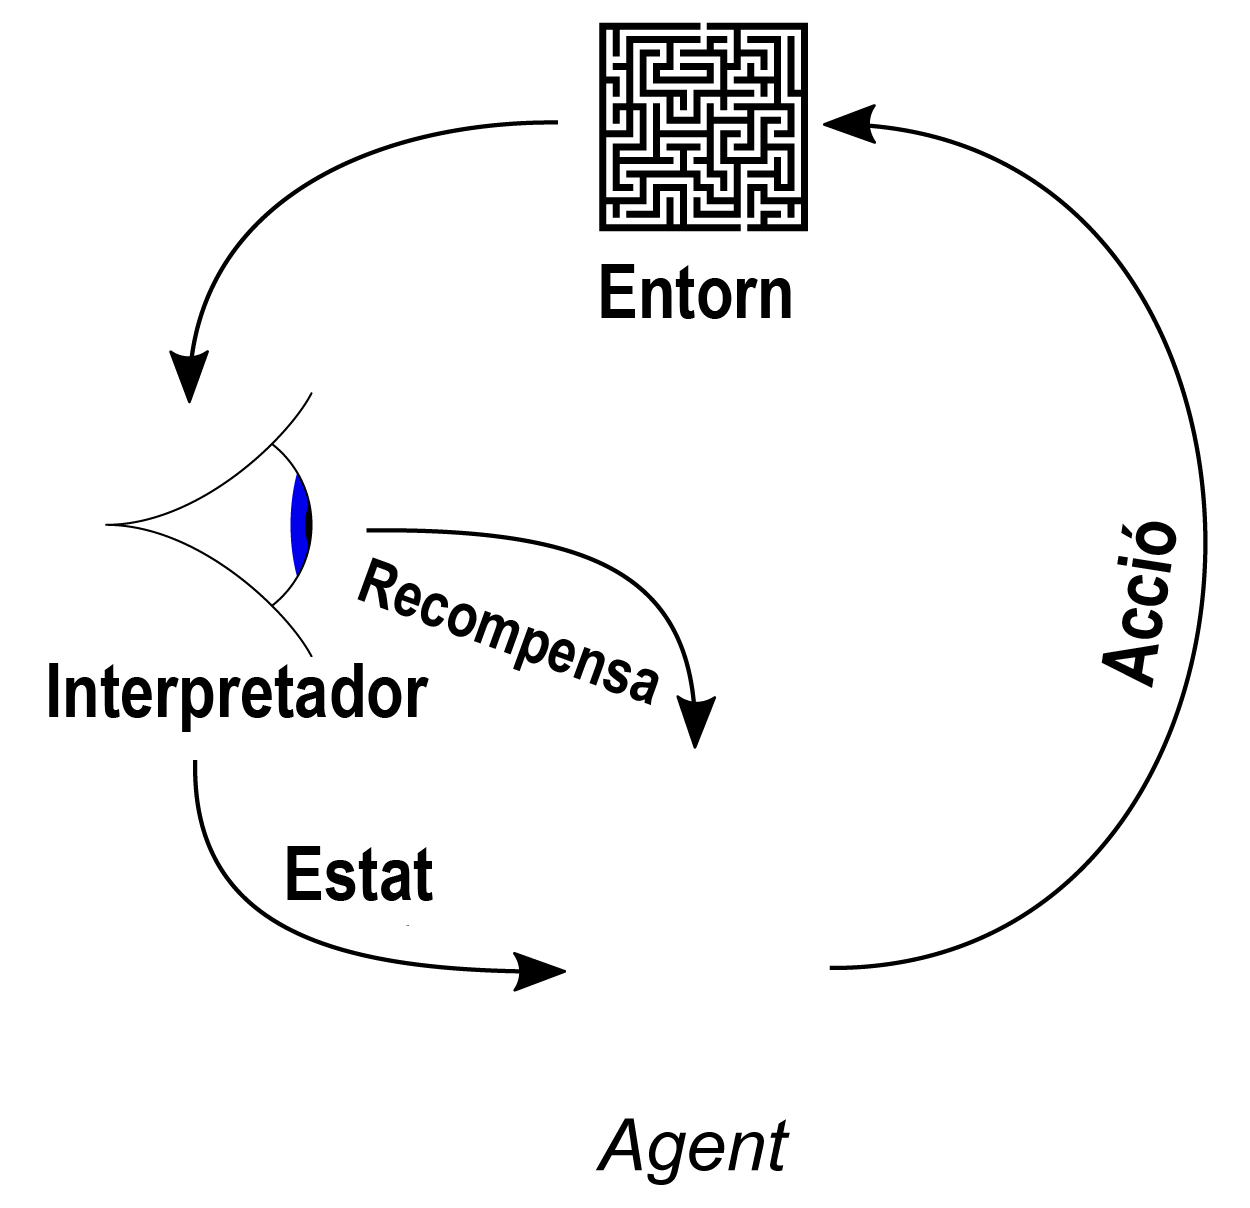
\includegraphics[width=8cm]{Reinforcement}
		\caption{Aprenentatge per reforçament}
		\label{fig:rein}
	\end{figure}
	
	\section{Aprenentatge profund}
	
	L'aprenentatge profund és una subcategoria d'aprenentatge automàtic. De forma similar a l'aprenentatge automàtic, l'aprenentatge profund també té l'aprenentatge supervisat, no supervisat i per reforç. Com s'ha comentat anteriorment, la idea de la IA es va inspirar en el cervell humà. Per tant, l’aprenentatge profund es va inspirar en xarxes neuronals artificials i les xarxes neuronals artificials es van inspirar en xarxes neuronals biològiques humanes. L'aprenentatge profund és una de les maneres d’executar l'aprenentatge automàtic.\supercite{DataCamp,dl}
	
	L'aprenentatge profund utilitza xarxes neuronals artificials amb diverses capes ocultes (\cref{fig:ann}) per extreure progressivament característiques o atributs de nivell superior a partir l’entrada. Per exemple, en el processament d’imatges, les capes inferiors poden identificar les vores, mentre que les capes superiors poden identificar els conceptes rellevants per a un humà com ara dígits, lletres o cares.\supercite{dlwiki}

	\addtocontents{toc}{\vspace{1em}}
	\printbibliography[heading=subbibintoc]

\end{refsection}

\newpage

\begin{refsection}

	\chapter{Xarxes neuronals artificials}
	\label{chap:ANN}

	El cervell és, sens dubte, l'òrgan més complex del nostre cos. El cervell humà és una xarxa neuronal biològica: una xarxa interconnectada de neurones que transmeten senyals elèctrics. Les neurones o cèl·lules nervioses són les unitats fonamentals del cervell i el sistema nerviós. Per les \textit{dendrites} (ramificacions nervioses), les neurones reben senyals d'entrada a través dels \textit{neurotransmissors} que alliberen els \textit{axons} d'altres cèl·lules nervioses i, quan els senyals rebuts són prou forts (superen un cert \textit{llindar}), les neurones s'activen i emeten un senyal de sortida a través d'un axó. L'impuls elèctric viatja al llarg de l'axó i provoca l'alliberament de neurotransmissors en la \textit{sinapsi}, que és el punt on es produeix aquest alliberament i la recepció del missatge per una altra neurona.\supercite{ANNBeginners} D'aquesta manera les neurones es poden comunicar entre elles. Tanmateix, el funcionament del cervell humà és un misteri molt més complex, que no s'explicarà en aquest treball.

	Les xarxes neuronals artificials (en endavant, xarxes neuronals) són un model d'aprenentatge automàtic inspirat en xarxes neuronals biològiques que formen els cervells dels humans i animals. Una xarxa neuronal està formada per un conjunt d'unitats o nodes connectats anomenats neurones artificials (en endavant, neurones) que simulen el funcionament de les neurones biològiques. A través de les connexions (sinapsis en les neurones biològiques) les neurones poden transmetre i rebre senyals d'altres neurones. Cada neurona rep una sèrie d'entrades, processa aquestes entrades i emet una sortida.\supercite{ANNFundamentals}

	\section{Perceptró}

	Per començar explicaré què és un perceptró. El perceptró és la xarxa neuronal més simple possible: un model computacional duna sola neurona. Els perceptrons van ser inventats i desenvolupats en els anys 1950 i 1960 per Frank Rosenblatt.\supercite{principles} Tanmateix, el principal model de neurones més utilitzat actualment és la \textit{neurona sigmoide}.

	Un perceptró rep diverses entrades, normalment binàries, en forma de vector $\vec{x}=(x_1,x_2,\ldots,x_{n-1},x_n)$, i produeix una única sortida binària $y$. La seva funció d'activació és la funció esglaó de Heaviside (\cref{fig:heaviside}).

	\begin{figure}[h]
		\centering
		\begin{minipage}[b]{.5\textwidth}
			\centering
			\begin{tikzpicture}
				[
					cmhplot/.style={color=red,mark=none,line width=1pt,<->},
					soldot/.style={color=red,only marks,mark=*},
					holdot/.style={color=red,fill=white,only marks,mark=*}
				]
				\begin{axis}
					\addplot[cmhplot,<-,domain=-3:0]{0};
					\addplot[cmhplot,->,domain=0:3]{1};
					\addplot[soldot]coordinates{(0,1)};
					\addplot[holdot]coordinates{(0,0)};
					\node [cmhplot] at (axis cs:0,0.5) {
						$H(x) =
							\begin{cases}
								1 & \text{si $x\geq 0$} \\
								0 & \text{si $x<0$}
							\end{cases}$
					};
				\end{axis}
			\end{tikzpicture}
			\captionof{figure}{Funció esglaó de Heaviside}
			\label{fig:heaviside}
		\end{minipage}%
		\begin{minipage}[b]{.5\textwidth}
			\centering
			\begin{tikzpicture}
				[x=1.5cm, y=1.5cm, >=stealth,
					neuron/.style={
							circle,
							draw,
							minimum size=1cm
						},
				]
				\node (in-1) at (0,1.5)  {$x_1$};
				\node (in-2) at (0,0.5)  {$x_2$};
				\node [draw=none, scale=2, text height=0.333cm] (in-m) at (0,0) {$\vdots$};
				\node (in-n-1) at (0,-0.5) {$x_{n-1}$};
				\node (in-n) at (0,-1.5) {$x_n$};

				[draw=none, scale=2, text height=0.333cm] (in-m) at

				\node [neuron] (neuron) at (2,0) {$b$};

				\node (out) at (4, 0) {$f(\vec{x})$};

				\draw [->] (neuron) -- (out);

				\draw [->] (in-1) -- (neuron)
				node [above, midway] {$w_1$};
				\draw [->] (in-2) -- (neuron)
				node [above, midway] {$w_2$};
				\draw [->] (in-n-1) -- (neuron)
				node [above, midway] {$w_{n-1}$};
				%\draw [->] (in-m) -- (neuron)
				%	node [above, midway] {$\ldots$};
				\draw [->] (in-n) -- (neuron)
				node [above, midway] {$w_n$};
			\end{tikzpicture}
			\captionof{figure}{Representació d'un perceptró}
			\label{fig:perceptron}
		\end{minipage}
	\end{figure}

	En la \cref{fig:perceptron} es mostra un perceptró amb $n$ entrades. A l'hora de calcular la sortida, el vector de pesos $\vec{w}=(w_1,w_2,\ldots,w_{n-1},w_n)$ expressa la importància de les respectives entrades per a la sortida. la qual depèn de si la suma ponderada $\sum_{i=1}^{n}w_ix_i$ és major o menor que el \textit{llindar}, un paràmetre real del perceptró,\supercite{nielsen} com es pot veure en l'\cref{eq:perceptron1}:

	\begin{equation}
		\label{eq:perceptron1}
		y=f(\vec{x})=
		\begin{cases}
			1 & \text{si $\sum_{i=1}^{n}w_ix_i\geq\mathrm{llindar}$} \\
			0 & \text{altrament}
		\end{cases}
	\end{equation}

	Per simplificar podem reescriure $\sum_{i=1}^{n}w_ix_i$ com un producte escalar de vectors, $\vec{w}\cdot\vec{x}\equiv\sum_{i=1}^{n}w_ix_i$. El llindar pot ser substituït pel \textit{biaix}, $b\equiv-\mathrm{llindar}$, que indica la facilitat del perceptró per  activar-se (emetre un $1$).\supercite{TDSperceptron2} L'\cref{eq:perceptron1} es pot expressar com:

	\begin{equation}
		\label{eq:perceptron2}
		y=f(\vec{x})=
		\begin{cases}
			1 & \text{si $\vec{w}\cdot\vec{x}+b\geq0$} \\
			0 & \text{altrament}
		\end{cases}
	\end{equation}

	\begin{comment}
	\begin{figure}[h]
		\centering
		\begin{tikzpicture}
			[x=1.5cm, y=1.5cm, >=stealth,
				every neuron/.style={
						circle,
						draw,
						minimum size=1cm
					},
				neuron missing/.style={
						draw=none,
						scale=4,
						text height=0.333cm,
						execute at begin node=\color{black}$\vdots$
					},
			]

			\foreach \m/\l [count=\y] in {1,2,3,missing,4}
			\node [every neuron/.try, neuron \m/.try] (input-\m) at (0,2.5-\y) {};

			\foreach \m [count=\y] in {1,missing,2}
			\node [every neuron/.try, neuron \m/.try ] (hidden-\m) at (2,2-\y*1.25) {};

			\foreach \m [count=\y] in {1,missing,2}
			\node [every neuron/.try, neuron \m/.try ] (output-\m) at (4,1.5-\y) {};

			\foreach \l [count=\i] in {1,2,3,n}
			\draw [<-] (input-\i) -- ++(-1,0)
			node [above, midway] {$I_\l$};

			\foreach \l [count=\i] in {1,n}
			\node [above] at (hidden-\i.north) {$H_\l$};

			\foreach \l [count=\i] in {1,n}
			\draw [->] (output-\i) -- ++(1,0)
			node [above, midway] {$O_\l$};

			\foreach \i in {1,...,4}
			\foreach \j in {1,...,2}
			\draw [->] (input-\i) -- (hidden-\j);

			\foreach \i in {1,...,2}
			\foreach \j in {1,...,2}
			\draw [->] (hidden-\i) -- (output-\j);

			\foreach \l [count=\x from 0] in {Input, Hidden, Ouput}
			\node [align=center, above] at (\x*2,2) {\l \\ layer};

		\end{tikzpicture}
		\caption{Example of a parametric plot ($\sin (x), \cos(x), x$)}
	\end{figure}
	\end{comment}

	\subsection{Interpretació gràfica}
	
	\begin{figure}[H]
		\centering
		\begin{tikzpicture}
		\begin{axis}[
		axis x line=center,
		axis y line=center,
		xmin=-0.1,xmax=1.2,
		ymin=-0.1,ymax=1.2,
		xlabel=$x_1$,
		ylabel=$x_2$,
		xtick={0,1},
		ytick={0,1},
		axis on top
		]
		\addplot[name path=e,color=red,mark=none,line width=1pt,domain=-0.6:1.8]{-0.45*x+0.5};
		\node at (axis cs:0.5,0.5) {$0.9x_1+2x_2\geq1$};
		\node at (axis cs:0.3,0.1) {$0.9x_1+2x_2<1$};
		
		\addplot[name path=u,draw=none]{-0.45*x+3};
		\addplot[name path=d,draw=none]{-0.45*x-3};
		
		\addplot[color=black!10] fill between[of=e and u];
		\addplot[color=black!20] fill between[of=e and d];
		
		\end{axis}
		\end{tikzpicture}
		\caption{La separació de l'espai d'entrada amb un perceptró}
		\label{fig:separation}
	\end{figure}
	
	Un perceptró separa l'espai d'entrada en dos semiespais. Per als punts que pertanyen a un semiespai el resultat del càlcul és $0$ i per als que pertanyen a l'altre, és $1$. La \cref{fig:separation} mostra la separació del pla en dos semiplans en el cas d'un perceptró de dues entrades, $x_1$ i $x_2$, amb $\mathrm{llindar}=1$, i pesos $w_1=0.9$ i $w_2=2$. És possible generar separacions arbitràries d'espai d'entrada ajustant els paràmetres d'aquest exemple.\supercite{Rojas1996}
	
	\subsection{Exemple pràctic}
	
	En resum, un perceptró és un dispositiu que pren decisions sospesant l'evidència.\supercite{MPerceptron1,nielsen} Intentem reproduir aquest procés de presa de decisions al món real. Suposem que vull veure un partit de futbol. Abans de prendre la decisió de reservar les entrades, tindria en compte diversos factors:

	\begin{enumerate}
		\item Hi juga el meu \textit{equip} preferit?
		\item El \textit{preu} de l'entrada és barat?
		\item El \textit{temps} és bo?
	\end{enumerate}

	Aquestes són els quatre factors (variables) a partir dels quals prendré la decisió. Són les entrades binàries $x_1,x_2,x_3$ per al perceptró, respectivament. Per exemple, tenim $x_1=1$ si m'agraden els equips que juguen, i $x_1=0$ si no m'agraden. De la mateixa manera, $x_2=1$ si l'entrada és barata, i $x_2=0$ si no ho és. I de manera similar per a $x_3$.

	Ara s'ha d'establir els pesos $w_1,w_2,w_3$. Els pesos relacionen cada entrada amb la de sortida corresponent. Suposem que adoro el futbol, de manera que estic encantat d'anar al festival, encara que faci mal temps i el preu de les entrades sigui car. Però sóc molt exigent amb els equips que hi juguen.

	Podem triar un pes $w_1=6$ per als equips, i $w_2=2$ i $w_3=2$ per als altres factors (\cref{fig:experceptron}). El valor més gran de $w_1$ i indica que els equips són molt importants per a mi, molt més que el temps i el preu. També establim un llindar mitjà de 5, $\mathrm{llindar}=5$, o un biaix de -5, $b=-5$.

	Ara avaluem els dos casos següents:

	\begin{itemize}

		\item El meu equip favorit juga, $x_1=1$; el preu de l'entrada és molt alt, $x_2=0$; el temps és molt dolent, $x_3=0$. Podem veure que el valor avaluat del model és $1$, superior a $0$ (\cref{eq:case1}). Per tant, la sortida del perceptró serà $1$ (\cref{eq:perceptron1}), que vol dir que aniré al partit (\cref{fig:experceptron1}).

		      \begin{equation}
			      \label{eq:case1}
			      \vec{w}\cdot\vec{x}+b=
			      w_1x_1+w_2x_2+w_3x_3+b=
			      6\cdot1+2\cdot0+2\cdot0-5=1>0
		      \end{equation}

		\item El meu equip favorit no juga, $x_1=0$; el preu de l'entrada és molt barat, $x_2=1$; el temps és bo, $x_3=1$. Podem veure que el valor avaluat del model és $-1$, inferior a $0$ (\cref{eq:case2}). Per tant, la sortida del perceptró serà $0$ (\cref{eq:perceptron1}), que vol dir que aniré al partit (\cref{fig:experceptron2}).

		      \begin{equation}
			      \label{eq:case2}
			      \vec{w}\cdot\vec{x}+b=
			      w_1x_1+w_2x_2+w_3x_3+b=
			      6\cdot0+2\cdot1+2\cdot1-5=-1<0
		      \end{equation}

	\end{itemize}

	\begin{figure}[H]
		\centering
		\begin{subfigure}[t]{0.5\textwidth}
			\centering
			\begin{tikzpicture}
				[x=1.5cm, y=1.5cm, >=stealth,
					neuron/.style={
							circle,
							draw,
							minimum size=1cm
						},
				]
				\node (in-1) at (0,1)  {$1$};
				\node (in-2) at (0,0)  {$0$};
				\node (in-3) at (0,-1) {$0$};

				\node [neuron] (neuron) at (2,0) {$-5$};

				\node (out) at (4, 0) {$1$};

				\draw [->] (neuron) -- (out);

				\draw [->] (in-1) -- (neuron)
				node [above, midway] {$6$};
				\draw [->] (in-2) -- (neuron)
				node [above, midway] {$2$};
				\draw [->] (in-3) -- (neuron)
				node [above, midway] {$2$};
			\end{tikzpicture}
			\caption{$\vec{x}=(1,0,0)$}
			\label{fig:experceptron1}
		\end{subfigure}%
		\begin{subfigure}[t]{0.5\textwidth}
			\centering
			\begin{tikzpicture}
				[x=1.5cm, y=1.5cm, >=stealth,
					neuron/.style={
							circle,
							draw,
							minimum size=1cm
						},
				]
				\node (in-1) at (0,1)  {$0$};
				\node (in-2) at (0,0)  {$1$};
				\node (in-3) at (0,-1) {$1$};

				\node [neuron] (neuron) at (2,0) {$-5$};

				\node (out) at (4, 0) {$0$};

				\draw [->] (neuron) -- (out);

				\draw [->] (in-1) -- (neuron)
				node [above, midway] {$6$};
				\draw [->] (in-2) -- (neuron)
				node [above, midway] {$2$};
				\draw [->] (in-3) -- (neuron)
				node [above, midway] {$2$};
			\end{tikzpicture}
			\caption{$\vec{x}=(0,1,1)$}
			\label{fig:experceptron2}
		\end{subfigure}
		\caption{Exemple d'un perceptró amb $\vec{w}=(6,2,2)$ i $b=-5$}
		\label{fig:experceptron}
	\end{figure}

	Com podem veure, amb aquests paràmetres el perceptró implementa un model de presa de decisions, que produeix un $1$ a la sortida sempre que hi jugui el meu equip preferit, i un $0$ sempre que no hi jugui. El preu de les entrades i el temps no influeixen en el resultat.

	Variant els pesos i el llindar, podem obtenir diferents models de presa de decisions. Per exemple, suposem que escollim un llindar de $3$. Aleshores, el perceptró decidirà que aniré a veure el partit quan hi jugui el meu equip preferit o quan tant el preu de l'entrada sigui barat i el temps sigui bo. És a dir, seria un model diferent de presa de decisions. Un llindar més petit significa que estic més disposat a anar al partit.\supercite{nielsen}
	
	\subsection{Xarxes de perceptrons}
	
	Evidentment, el perceptró no és un model complet de presa de decisions humanes, però el que ens mostra l'exemple anterior és la capacitat d'un perceptró de prendre decisions simples. Per tant, sembla plausible que una xarxa complexa de perceptrons (\cref{fig:ann}) pugui prendre decisions molt subtils.\supercite{MPerceptron1}

	\begin{figure}[h]
		\centering
		\begin{comment}
		\begin{tikzpicture}[x=1.5cm, y=1.5cm, >=stealth,
				every neuron/.style={
					circle,
					draw,
					minimum size=1cm
				},
			]

			\foreach \m/\l [count=\y] in {1,...,4}
			\node [every neuron/.try, neuron \m/.try] (input-\m) at (0,2-\y) {$x_\m$};

			\foreach \m [count=\y] in {1,...,5}
			\node [every neuron/.try, neuron \m/.try ] (hidden1-\m) at (2,2.5-\y) {};
			
			\foreach \m [count=\y] in {1,...,4}
			\node [every neuron/.try, neuron \m/.try ] (hidden2-\m) at (4,2-\y) {};

			\foreach \m [count=\y] in {1,...,3}
			\node [every neuron/.try, neuron \m/.try ] (output-\m) at (6,1.5-\y) {};

			%\foreach \l [count=\i] in {1,2,3,n}
			%\draw [<-] (input-\l) -- ++(-1,0)
			%node [above, midway] {$x_\l$};

			%\foreach \l [count=\i] in {1,n}
			%\node [above] at (hidden1-\i.north) {$H_\l$};

			\foreach \l [count=\i] in {1,...,3}
			\draw [->] (output-\i) -- ++(1,0)
			node [above, midway] {$O_\l$};

			\foreach \i in {1,...,6n}
			\foreach \j in {1,...,5}
			\draw [->] (input-\i) -- (hidden1-\j);
			
			\foreach \i in {1,...,5}
			\foreach \j in {1,...,4}
			\draw [->] (hidden1-\i) -- (hidden2-\j);

			\foreach \i in {1,...,4}
			\foreach \j in {1,...,3}
			\draw [->] (hidden2-\i) -- (output-\j);

			\foreach \l [count=\x from 0] in {Input, Hidden, Hidden, Ouput}
			\node [align=center, above] at (\x*2,3) {\l \\ layer L_{\l+1};
		\end{tikzpicture}
		\end{comment}
		
		\begin{neuralnetwork}[height=4,nodesize=1cm,nodespacing=1.5cm,layertitleheight=5em]
			\newcommand{\nodetextclear}[2]{}
			\newcommand{\nodetextx}[2]{$x_#2$}
			\newcommand{\nodetexty}[2]{$y_#2$}
			\inputlayer[count=4, bias=false, title={Capa\\d'entrada $L_1$}, text=\nodetextx]
			\hiddenlayer[count=5, bias=false, title={Capa\\oculta $L_2$}, text=\nodetextclear] \linklayers
			\hiddenlayer[count=5, bias=false, title={Capa\\oculta $L_3$}, text=\nodetextclear] \linklayers
			\outputlayer[count=3, title={Capa\\de sortida $L_4$}, text=\nodetexty] \linklayers
		\end{neuralnetwork}
		
		\caption{Xarxa de perceptrons}
		\label{fig:ann}
	\end{figure}

	Les entrades $x_1,x_2,\ldots$ es poden representar com a variables flotant a l’esquerra de la xarxa de perceptrons (\cref{fig:perceptron}), però és convencional dibuixar una capa addicional de perceptors (la capa d’entrada $L_1$, \cref{fig:ann}) per codificar les entrades. Els perceptrons d'entrada realment no són perceptrons, sinó unitats especials que simplement emeten els valors desitjats $x_1,x_2,\ldots$.
	
	\subsection{Aprenentage del perceptró}
	
	Ara ens podem fer dues preguntes senzilles:
	
	\begin{itemize}
		\item Com seleccionar els valors dels pesos? Als exemples anteriors, aquests valors s'introdueixen manualment, però les xarxes neuronals no funcionen d'aquesta manera.
		
		\item Com seleccionar el valor del llindar o del biaix?
	\end{itemize}

	Es poden dissenyar \textit{algoritmes d'aprenentatge} que puguin ajustar automàticament els pesos i els biaixos d'una xarxa de neurones artificials. Aquest ajustament es produeix en resposta als estímuls externs, sense intervenció directa d'un programador. Els algoritmes d'aprenentatge permeten a les xarxes neuronals aprendre a resoldre problemes. Però, com podem elaborar aquests algoritmes?
	
	Suposem que tenim una xarxa de perceptors que volem utilitzar per aprendre a resoldre algun problema. Per exemple, les entrades a la xarxa poden ser els píxels d'una imatge manuscrita d'un dígit. I volem que la xarxa aprengui els pesos i els biaixos per obtenir a la seva sortida una classificació correcta del dígit. Per veure com pot funcionar l'aprenentatge, suposem que fem un petit canvi en algun pes (o biaix) a la xarxa. El que volem és que aquest petit canvi de pes causi només un petit canvi corresponent en la sortida de la xarxa (\cref{fig:learn}). Aquesta propietat farà possible l'aprenentatge.
	
	\begin{figure}[h]
		\centering
		\begin{tikzpicture}[x=1.5cm, y=1.5cm, >=stealth,
			every neuron/.style={
				circle,
				draw,
				minimum size=1cm
			},
		]
			\foreach \m/\l [count=\y] in {1,...,3}
			\node [every neuron/.try, neuron \m/.try] (input-\m) at (0,2-\y) {};
		
			\foreach \m [count=\y] in {1,...,4}
			\node [every neuron/.try, neuron \m/.try ] (hidden1-\m) at (2,2.5-\y) {};
		
			\foreach \m [count=\y] in {1}
			\node [every neuron/.try, neuron \m/.try ] (output-\m) at (4,1-\y) {};
		
			%\foreach \l [count=\i] in {1,2,3,n}
			%\draw [<-] (input-\l) -- ++(-1,0)
			%node [above, midway] {$x_\l$};
		
			%\foreach \l [count=\i] in {1,n}
			%\node [above] at (hidden1-\i.north) {$H_\l$};
		
			\foreach \l [count=\i] in {1}
			\draw [->] (output-\i) -- ++(1,0);
			
			\node [align=center] at (5.5,0) {$y+\Delta y$};
		
			\foreach \i in {1,...,3}
			\foreach \j in {1,...,4}
			\draw [->] (input-\i) -- (hidden1-\j);
			
			\foreach \i in {1,...,4}
			\foreach \j in {1}
			\draw [->] (hidden1-\i) -- (output-\j);
			
			%\foreach \l [count=\x from 0] in {Input, Hidden, Ouput}
			%\node [align=center, above] at (\x*2,2.5) {\l \\ layer};
			\node [align=center, above] at (1,1.5) {$w+\Delta w$};
		\end{tikzpicture}
		\caption{Aprentatge d'una xarxa de perceptrons}
		\label{fig:learn}
	\end{figure}

	Si és cert que un petit canvi en un pes (o biaix) provoca només un petit canvi en la sortida, podem utilitzar aquest fet per modificar els pesos i els biaixos per aconseguir que la xarxa es comport de la manera que desitgem. Per exemple, suposem que la xarxa classificava erròniament una imatge com a $8$ quan hauria de ser un $9$. Podríem esbrinar com es pot fer un petit canvi en els pesos i els biaixos, de manera que la xarxa s'acosti una mica més a la correcta classificació de la imatge. I després repetiríem això, canviant els pesos i els biaixos una vegada darrere l'altra per aconseguir cada cop millors resultats. La xarxa estaria aprenent.
	
	El problema és que això no passa amb perceptrons. Així doncs, un petit canvi en els pesos o biaixos d'un sol perceptró d'una xarxa fa que la sortida d'aquesta passi de $0$ a $1$ i viceversa, canviant el comportament de la xarxa de forma molt aleatòria, ja que el perceptró replica una funció esglaó (\cref{fig:heaviside}). Això fa que sigui difícil veure com modificar gradualment els pesos i els biaixos de manera que la xarxa s’acosti al comportament desitjat.
	
	Podem superar aquest problema introduint un nou tipus de neurona artificial anomenada \textit{neurona sigmoide}.
	
	\section{Neurona sigmoide}
	
	Les neurones sigmoides són similars als perceptrons, però es modificades de tal manera que els petits canvis en els seus pesos i biaixos causen només un petit canvi en la seva sortida. Aquest fet permetrà aprendre a una xarxa de neurones sigmoides.\supercite{TDSsigmoid}
	
	Les neurones sigmoides es representen de la mateixa manera que els perceptrons (\cref{fig:neuron}).
	
	\begin{figure}[h]
		\centering
		\begin{tikzpicture}
		[x=1.5cm, y=1.5cm, >=stealth,
		neuron/.style={
			circle,
			draw,
			minimum size=1cm
		},
		]
		\node (in-1) at (0,1.5)  {$x_1$};
		\node (in-2) at (0,0.5)  {$x_2$};
		\node [draw=none, scale=2, text height=0.333cm] (in-m) at (0,0) {$\vdots$};
		\node (in-n-1) at (0,-0.5) {$x_{n-1}$};
		\node (in-n) at (0,-1.5) {$x_n$};
		
		[draw=none, scale=2, text height=0.333cm] (in-m) at
		
		\node [neuron] (neuron) at (2,0) {$b$};
		
		\node (out) at (4, 0) {$f(\vec{x})$};
		
		\draw [->] (neuron) -- (out);
		
		\draw [->] (in-1) -- (neuron)
		node [above, midway] {$w_1$};
		\draw [->] (in-2) -- (neuron)
		node [above, midway] {$w_2$};
		\draw [->] (in-n-1) -- (neuron)
		node [above, midway] {$w_{n-1}$};
		%\draw [->] (in-m) -- (neuron)
		%	node [above, midway] {$\ldots$};
		\draw [->] (in-n) -- (neuron)
		node [above, midway] {$w_n$};
		\end{tikzpicture}
		\captionof{figure}{Representació d'una neurona sigmoide}
		\label{fig:neuron}
	\end{figure}

	Igual que un perceptró, la neurona sigmoide té diverses entrades reals, $x_1,x_2,\ldots$, pesos per a cada entrada, $w_1,w_2,\ldots$ i un biaix, $b$. Però la seva sortida no és binària ($0$ o $1$). En canvi, la sortida d'una neurona sigmoide és $\sigma(\vec{w}\cdot\vec{x}+b)$, on $\sigma$ s'anomena \textit{funció sigmoide} (\cref{eq:sigmoid}, \cref{fig:sigmoid}). La funció $\sigma$ també es diu \textit{funció logística} i les neurones es diuen \textit{neurones logístiques}.
	
	\begin{equation}
		\label{eq:sigmoid}
		\sigma(x)=\frac{1}{1+e^{-x}}
	\end{equation}
	
	\begin{figure}[H]
		\centering
	\begin{tikzpicture}
	[
	cmhplot/.style={color=red,mark=none,line width=1pt},
	]
	\begin{axis}[
	grid=both,
	xmin=-6,xmax=6,
	ymin=0,ymax=1
	]
	\addplot[cmhplot,domain=-6:6]{1/(1+exp(-x))};
	%\node [cmhplot] at (axis cs:0,0.5) {
	%	$H(x) =
	%	\begin{cases}
	%	1 & \text{si $x\geq 0$} \\
	%	0 & \text{si $x<0$}
	%	\end{cases}$
	%};
	\end{axis}
	\end{tikzpicture}
	\captionof{figure}{Funció sigmoide}
	\label{fig:sigmoid}
	\end{figure}

	En aquest cas, la funció sigmoide és la \textit{funció d'activació} o \textit{funció de transferència} de la neurona sigmoide. En el cas del perceptró, la seva funció d'activació és la funció esglaó $H(x)$ i la sortida $f(\vec{x})=H(\vec{w}\cdot\vec{x}+b)$. Per a qualsevol altra funció d'activació $g(x)$ la sortida de la neurona serà $f(\vec{x})=g(\vec{w}\cdot\vec{x}+b)$.

	Per tant, la sortida d'una neurona sigmoide amb entrades $\vec{x}=(x_1,x_2,\ldots)$, pesos $\vec{w}=(w_1,w_2,\ldots)$ i biaix $b$ és:
	
	\begin{equation}
		\label{eq:out}
		f(\vec{x})=\sigma(\vec{w}\cdot\vec{x}+b)=\frac{1}{1+e^{-(\vec{w}\cdot\vec{x}+b)}}
	\end{equation}

	La forma de la funció sigmoide (\cref{fig:sigmoid}) és una versió suavitzada de la funció esglaó (\cref{fig:heaviside}). La suavitat de $\sigma$ significa que petits canvis $\Delta w_i$ en els pesos i $\Delta b$ en el biaix produiran un petit canvi $\Delta y$ en la sortida de la neurona, propietat necessària perquè la xarxa pugui aprendre.
	
	\addtocontents{toc}{\vspace{1em}}

	\printbibliography[heading=subbibintoc]

\end{refsection}

\newpage

\begin{refsection}

	\chapter{Disseny i programació de xarxes neuronals}
	\label{chap:pract}

	La finalitat del treball és l'aplicació dels conceptes de xarxes neuronals. Es provaran xarxes neuronals simples amb diferents funcions d'activació per veure el seu comportament i la seva precisió. Com a base del projecte, s'ha utilitzat la base de dades \textbf{MNIST}, \cref{fig:mnist}, un conjunt d'imatges de dígits escrits a mà que són emprats per a l'entrenament de sistemes de classificació automàtica d'imatges. És l'evolució de la base de dades NIST. MNIST consta d'un conjunt de 70000 dígits manuscrits: 60000 imatges per entrenar la xarxa neuronal i 10000 imatges per mesurar la seva eficiència.\supercite{MNIST}
	
	\begin{figure}[h]
		\centering
		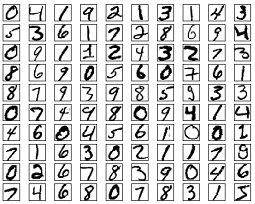
\includegraphics[width=8cm]{mnist}
		\caption{Base de dades MNIST}
		\label{fig:mnist}
	\end{figure}

	Pel que fa a les tecnologies i \textit{frameworks} d'aprenentatge profund, hi ha diverses eleccions a considerar: \textbf{TensorFlow}, \textbf{Keras}, \textbf{PyTorch}:
	
	\begin{itemize}
		\item \textbf{TensorFlow} és una biblioteca de programari de codi obert per a l'aprenentatge profund i automàtic desenvolupada per l'equip Google Brain per satisfer les seves necessitats de crear i entrenar xarxes neuronals per detectar i desxifrar patrons i correlacions. S'utilitza tant per a la investigació com per a la producció a Google i està sota la llicència Apache 2.0.\supercite{TensorFlow}
		
		En aquest projecte s'utilitzarà TensorFlow per la seva capacitat per realitzar un bon rendiment a càlculs de nivell baix i alt. També, a causa de la naturalesa de processament d'imatges del projecte i la seva capacitat d'integració fàcil amb altres biblioteques Python com NumPy\supercite{NumPy} o PIL.\supercite{Pillow}
		
		\item \textbf{Keras} és una biblioteca de xarxes neuronals de codi obert escrita en llenguatge Python. Keras es pot executar damunt de TensorFlow, Microsoft Cognitive Toolkit (CNTK) o Theano. Va ser desenvolupat per l'experimentació en xarxes neuronals. Els seus advantages són la facilitat d'ús, modularitat i extensibilitat.\supercite{Keras}
		
		\item \textbf{PyTorch} és una biblioteca de programari de codi obert per a l'aprenentatge automàtic, basada en la biblioteca Torch i escrita en Python, C++ i CUDA. És desenvolupada principalment pel grup de recerca d'intel·ligència artificial de Facebook.\supercite{PyTorch}
		
		
	\end{itemize}

	Com ja s'ha indicat anteriorment, un dels objectius del treball és aconseguir un valor de precisió el més proper al $100\%$ possible. Això s'aconsegueix mitjançant la configuració ideal de les variables com ara els pesos o els biaixos.
	
	L'activitat consisteix en programar una xarxa neuronal en la qual la sortida generada sigui el valor del número que la xarxa ha obtingut com a entrada però en format d’imatge. Ès a dir, la xarxa ha d'endevinar quin es el número escrit a mà. Com més encerti, obtindrà un valor de precisió o més
	elevat.
	
	Per aconseguir aquests valors, es diferencien dues fases de modelització
	
	\begin{itemize}
		\item \textit{Fase d’entrenament}. En aquesta fase s’utilitza una part
		del conjunt de dades (MNIST en aquest cas) per determinar els pesos que defineixen el model de la xarxa neuronal. Aquests pesos es calculen de manera iterativa, amb l'objectiu de minimitzar l'error obtingut entre la sortida resultant de la xarxa i el valor de sortida desitjat.
		
		Un altre concepte que s'utilitza en l'entrenament consisteix en la \textit{retropropagació} o \textit{backpropagation}.\supercite{backprop} És un metode de càlcul de pesos que s'utilitza en algoritmes d'aprenentatge i que ofereix molt bons resultats gràcies al reajustament dels pesos de les neurones en direcció contrària després d’haver recorregut la xarxa des del principi fins al final.
		
		Durant aquesta fase, el model pot patir un \textit{sobreentrenament}, de manera que s’ajusta massa a les particularitats del patró d'entrenament. En aquest cas es perdria l'habilitat de generar el seu aprenentatge en nous casos amb altres dades.
		
		\item \textit{Fase de prova}. Per evitar el problema del sobreentrenament, s'utilitza un segon
		grup de dades diferents de les d'entrenament per permetre controlar el procés d'aprenentatge.
		
		Aquest grup de dades s'utilitza per veure com reacciona el model davant dades que no ha analitzat anteriorment i es pot saber quin és el seu grau de precisió i el seu grau d'error.

	\end{itemize}

	El primer pas en el desenvolupament del projecte consisteix en crear una xarxa neuronal bàsica d'una sola capa. Aquesta vindria representada per 784 unitats d'entrada, que corresponen al nombre de píxels que conté la imatge del model de dades (24x24 píxels), i 10 sortides, que representen els deu possibles dígits $[0 - 9]$ de la imatge d'entrada.
	
	\begin{figure}[h]
		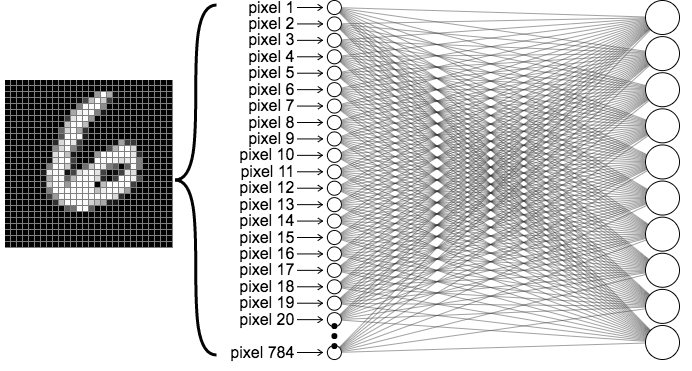
\includegraphics[width=\textwidth]{mnist1layer}
		\caption{Xarxa bàsica per MNIST\protect\supercite{Ml4a}}
	\end{figure}

	\section{Entorn}
	
	Primer de tot, cal destacar l’entorn dels experiments, tant el \textit{hardware} com el \textit{software}:
	
	\begin{itemize}
		\item CPU: Intel Core i7-8750H
		\item GPU: NVIDIA GeForce GTX 1060
		\item RAM: 16 GB DDR4
		\item OS: Windows 10
		\item \textbf{Python}. És un dels llenguatges de programació més utilitzats per experiments amb IA. És un llenguatge multiplataforma, orientat a objectes i fàcil d'aprendre gràcies a la seva sintaxi. Ha estat escollit per la gran quantitat de biblioteques, tipus de dades i funcions
		incorporades en el mateix llenguatge, que ajuden a realitzar moltes tasques sense necessitat de programar-les de zero.\supercite{Python}
		\item \textbf{TensorFlow}. Un dels \textit{frameworks} més utilitzats per realitzar la gestió de xarxes neuronals.\supercite{TDS10}
		\item \textbf{Keras}. S'executa per damunt de TensorFlow. Biblioteca de Python que proporciona, d'una manera simple i eficient, la creació de models de xarxes neuronals.\supercite{Keras,TDS10}
		\item \textbf{Anaconda}. És una distribució de codi obert dels llenguatges de programació Python.\supercite{Anaconda}
		\item \textbf{Jupyter Notebook}. És un entorn computacional interactiu basat en la web per crear documents de quaderns Jupyter (\textit{notebooks}) en llenguatge Python.\supercite{Jupyter}
	\end{itemize}

	\section{Xarxa neuronal}
	
	El primer pas realitzat consisteix en carregar el model de dades MNIST explicat anteriorment per a poder tractar-lo. Keras ja incorpora el conjunt de dades MNIST i només cal importar-lo i guardar-lo en les variables d'entrenament i test. Un cop fet, només cal preprocessar correctament les dades carregades d'aquest conjunt, com es mostra en el \cref{lst:first}.
	
	En aquest punt, tenim 60000 mostres de dígits del 0 al 9, escrits a mà, en una variable llesta per ser tractada per la xarxa que es crea a continuació.
	
	\begin{listing}[H]
		\begin{pythoncode}
# TensorFlow
import tensorflow as tf
# Model Sequential, pila lineal de capes de xarxes neuronals
from tensorflow.keras.models import Sequential
# Capes bàsiques de Keras
from tensorflow.keras.layers import Dense, Dropout, Activation, Flatten
# Utilities
from tensorflow.python.keras.utils import to_categorical

# Importar el conjunt de dades MNIST i guardar-lo en variables
from tensorflow.python.keras.datasets import mnist
(X_train, y_train), (X_test, y_test) = mnist.load_data()

# Preprocessar les dades
X_train = X_train.reshape(X_train.shape[0], 784)
X_test = X_test.reshape(X_test.shape[0], 784)
X_train = X_train.astype('float32')
X_test = X_test.astype('float32')
# Normalitzar els valors a l'interval [0, 1]
X_train /= 255
X_test /= 255
# Obtenir 10 classes per als dígits 0-9
Y_train = to_categorical(y_train, 10)
Y_test = to_categorical(y_test, 10)
\end{pythoncode}
		\caption{Importar MNIST i preprocessar les dades}
		\label{lst:first}
	\end{listing}

	El següent pas consisteix en la creació del model de la xarxa (\cref{lst:model}). Primerament, s’ha creat una xarxa amb estructura bàsica on les entrades es connecten directament amb les 10 neurones de sortida (una per cada dígit del 0 al 9, \cref{fig:mnistann1}). Seguidament es fa la compilació i lentrenament de la xarxa.

	\begin{listing}[H]
		\begin{pythoncode}
# Model
model = Sequential()
model.add(Dense(10, activation='sigmoid', input_shape=(784,)))

# Compilació del model
model.compile(loss='binary_crossentropy',
			  optimizer='adam', metrics=['accuracy'])

# Entrenament
hist = model.fit(X_train, Y_train,
				validation_data=(X_test, Y_test),
				epochs=20, verbose=1)
\end{pythoncode}
		\caption{Model de xarxa neuronal}
		\label{lst:model}
	\end{listing}
	
	\begin{figure}[H]
		\centering
		\begin{tikzpicture}[x=1.5cm, y=1.5cm, >=stealth,
		every neuron/.style={
			circle,
			draw,
			minimum size=1cm
		},
		neuron missing/.style={
			draw=none, 
			scale=4,
			text height=0.333cm,
			execute at begin node=\color{black}$\vdots$
		},
		]
		
		\foreach \m/\l [count=\y] in {1,2,3,missing,4}
		\node [every neuron/.try, neuron \m/.try] (input-\m) at (0,2.5-\y) {};
		
		\foreach \m [count=\y] in {1,missing,2}
		\node [every neuron/.try, neuron \m/.try ] (output-\m) at (2,1.5-\y) {};
		
		\foreach \l [count=\i] in {0,9}
		\draw [->] (output-\i) -- ++(1,0)
		node [above, midway] {$O_\l$};
		
		\foreach \i in {1,...,4}
		\foreach \j in {1,...,2}
		\draw [->] (input-\i) -- (output-\j);
		
		\node [align=center, above] at (0,2) {Capa d'entrada\\(784)};
		\node [align=center, above] at (2,2) {Capa de sortida\\(10)};
		\end{tikzpicture}
		\caption{Xarxa neuronal}
		\label{fig:mnistann1}
	\end{figure}

	El model creat representa un model seqüencial amb 784 entrades per una capa de 10 sortides i una funció d'activació sigmoide presentada anteriorment.
	
	Fins ara, hem aconseguit construir una xarxa neuronal capaç d'identificar dígits del 0 al 9 amb un percentatge d'encert prou alt. La \cref{fig:acc1,fig:loss1} mostra els resultats obtinguts mitjançant aquesta xarxa. Es poden observar dos gràfics que representen els valors \textit{accuracy} (precisió) i \textit{loss} (error) respecte les \textit{epochs}, és a dir, el percentatge d'encert i el valor d'error respecte a cada iteració del model.
	
	\begin{figure}[H]
		\centering
		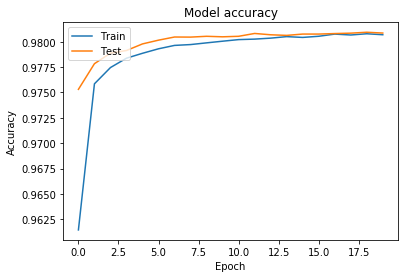
\includegraphics[width=.75\textwidth]{acc1}
		\captionof{figure}{Precisió de la xarxa}
		\label{fig:acc1}
	\end{figure}

	\begin{figure}[H]
		\centering
		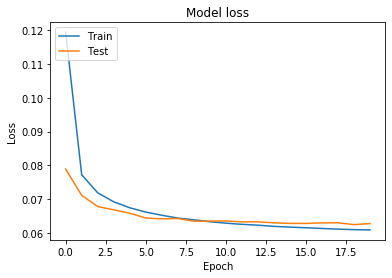
\includegraphics[width=0.75\textwidth]{loss1}
		\captionof{figure}{Error de la xarxa}
		\label{fig:loss1}
	\end{figure}

	Les modificacions posteriors de la xarxa neuronal amb la finalitat d'aconseguir més eficiència i l'applicació amb GUI (\cref{fig:app1,fig:app2}) es poden trobar a \cite{mygithub}.
	
	\begin{figure}[H]
		\centering
		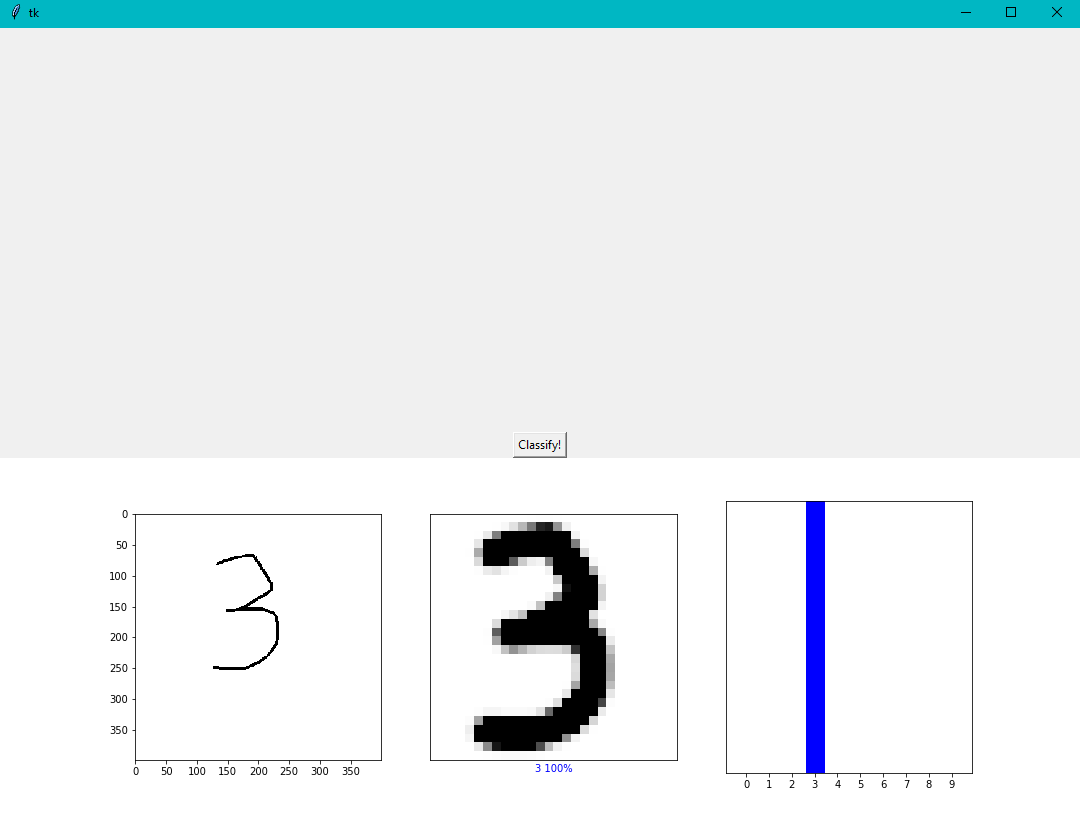
\includegraphics[width=.75\textwidth]{app3}
		\captionof{figure}{Applicació GUI}
		\label{fig:app1}
	\end{figure}

	\begin{figure}[H]
		\centering
		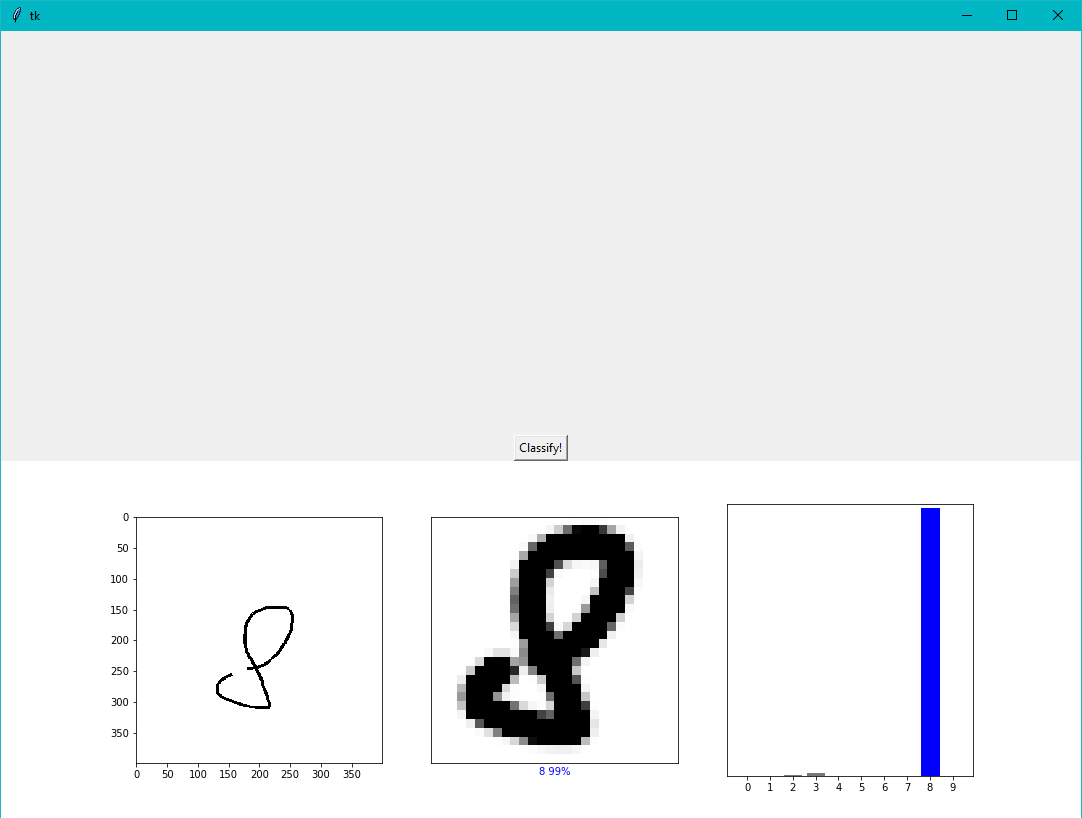
\includegraphics[width=.75\textwidth]{app8}
		\captionof{figure}{Applicació GUI}
		\label{fig:app2}
	\end{figure}

	\addtocontents{toc}{\vspace{1em}}
	\printbibliography[heading=subbibintoc]

\end{refsection}

\newpage

\begin{refsection}

	\chapter{Conclusió}
	\label{chap:conc}

	Com hem pogut observar, les xarxes neuronals proporcionen un gran potencial davant la resolució de problemes de predicció i classificació. En aquest cas, s’ha construït un model capaç de resoldre un problema relativament senzill per un ésser humà, però assolint amb un percentatge d'encert molt elevat.
	
	Tenint en compte que el problema resolt es considera senzill i introductori, la seva resolució il·lumina la idea sobre la diversitat dels problemes que es poden arribar a solucionar mitjançant l'aplicació de les xarxes neuronals en qualsevol context.
	
	Tot i això, les aplicacions que es poden extrapolar del model generat podrien arribar a ser molt útils i amb una bona acceptació comercial.
	
	Pel que fa als objectius fixats al començament del projecte, s'assoleix completament el propòsit principal de dissenyar i programar un model basat en xarxes neuronals capaç de reconèixer
	dígits escrits a mà amb una eficiència elevada.
	
	Aquest treball ha complert definitivament els seus objectius, no només cap a la familiarització amb conceptes de la intel·ligència artificial i aprenentatge automàtic aplicats al processament d'imatges, que és un camp que evoluciona constantment, sinó també s'ha après a dissenyar models de xarxes neuronals per al processament i reconeixement d'imatges.
	
	Afrontar problemes comuns en aquest àmbit com ara triar el \textit{framework} més adequat, triar el mètode d'optimització més eficaç, tractar les dades abans i després del processament, intentar esbrinar el millor mètode d'anàlisi per als resultats, solucionar problemes d'execució derivats de mal funcionament o optimitzar el model, són habilitats útils i de difícil adquisició.
	
	\begin{itemize}
		
		\item Hem aprendre conceptes que poden ser aplicats en diferents àrees com l'anàlisi d'imatges o presa de decisions.
		
		\item Explicar el funcionament de diferents mètodes d'aprenentatge automàtic (centrant-se principalment en les xarxes neuronals).
		
		\item Demostrar que els sistemes d'aprenentatge automàtic són útils i aplicables.
		
		\item Comprendre els conceptes, el funcionament i l'abast de les xarxes neuronals i mostrar el procés de disseny i implementació de xarxes neuronals amb TensorFlow i Keras per aconseguir objectius específics.
		
	\end{itemize}
	
	Reconeixement d'imatges (visió artificial):
	
	\begin{itemize}
		
		\item Dissenyar i implementar un model predictiu eficaç en la classificació de dígits escrits a mà utilitzant el conjunt de dades MNIST.
		
		\item Analitzar el funcionament i el rendiment de diferents arquitectures de xarxes neuronals.
		
	\end{itemize}
	
	\addtocontents{toc}{\vspace{1em}}
	\printbibliography[heading=subbibintoc]

\end{refsection}

\newpage

\begin{appendices}
	\begin{refsection}
\chapter{Desenvolupament del treball}

	En el primer bloc de la memòria s'ha explicat la part més teòrica del treball que consta de 3 apartats: \nameref{chap:AI}, \nameref{chap:ML} i \nameref{chap:ANN}. Aquesta part del treball inclou la recerca d'informació i, quan sigui possible, alguns exemples pràctics per complementar la teoria. En la recerca bibliogràfica s'han utilitzat diverses fonts:

	\begin{itemize}

		\item Com és natural, la font d'informació que més he utilitzat, la que predominarà en la part teòrica del treball i la que m’ha clarificat més conceptes ha estat la recerca amb els buscadors d'Internet. Per aquesta font he aconseguit molts treballs relacionats amb la intel·ligència artificial i l'aprenentatge automàtic. Entre els diferents treballs, destaquen els treballs de fi de grau (TFG) i els projectes de final de carrera (PFC) en l'àmbit de les Tecnologies de la Informació i les Comunicacions, sobretot l'Enginyeria Informàtica. Principalment, tota la informació d'aquesta font és en idioma anglès i extreta dels repositoris o dipòsits digitals de les universitats, com ara la UPF\supercite{eRepositoriUPF}, la UAB\supercite{DDDUAB} o la UPC.\supercite{UPCommons}

		\item A parts dels repositoris, he fet servir bases de dades d'autors i d'articles publicats a revistes científiques internacionals, amb l'ajuda del motor de cerca Google Acadèmic. M'agradaria destacar algunes pàgines web que m'han resultat molt útils:

		      \begin{itemize}

			      \item \textbf{Google Acadèmic} és un motor de cerca de Google que indexa el text complet o les metadades de literatura científico-acadèmica de gran quantitat de formats i disciplines.\supercite{GoogleScholar}

			      \item \textbf{Microsoft Academic} és un motor de cerca web públic i gratuït per a publicacions acadèmiques, desenvolupat per Microsoft Research.\supercite{MicrosoftAcademic}

			      \item \textbf{ResearchGate} és una xarxa social i una eina de col·laboració per a científics i investigadors per compartir documents, fer i respondre preguntes, i trobar col·laboradors.\supercite{ResearchGate}

			      \item \textbf{arXiv} és un repositori científic per a la publicació d'articles científics en format digital en els camps de les matemàtiques, física, informàtica i biologia que poden ser obtinguts lliurement a través d'Internet.\supercite{ArXiv}

		      \end{itemize}

		\item Gran part de la informació per dur a terme el disseny i la programació dels diferents models de xarxes neuronals en la part pràctica del treball són de fonts lliures. Això vol dir que aquesta informació s'ha obtingut de fòrums, blocs i pàgines web amb tutorials on els autors exposen, expliquen i mostren com fer determinades coses, sense un ànim de lucre. Comparteixen els seus mètodes i les seves conclusions de forma desinteressada. Això implica provar i verificar molts dels mètodes per assegurar el seu funcionament. Per tant, són referències a pàgines web actives i que poden modificar-se i desaparèixer en el temps. Concretament he utilitzat:

		      \begin{itemize}

			      \item \textbf{GitHub} és un servei de hosting de repositoris Git, el qual ofereix tota la funcionalitat de Git de control de revisió distribuït i administració de codi de la font (SCM) així com afegint les seves característiques pròpies.\supercite{GitHub}

			      \item \textbf{Stack Overflow} és una pàgina web de preguntes i respostes per a programadors professionals i entusiastes que forma part de la Xarxa Stack Exchange.\supercite{StackOverflow}

			      \item \textbf{Tutorials Point} és una pàgina web que ofereix una gran quantitat de tutorials, cursos i articles gratuïts relacionats amb temes de llenguatges de programació i altres tecnologies.\supercite{TutorialsPoint}

			      \item \textbf{Medium} és un servei de publicació de blogs.\supercite{Medium}

		      \end{itemize}

	\end{itemize}

	\addtocontents{toc}{\vspace{1em}}
	\printbibliography[heading=subbibintoc]

\end{refsection}
	\begin{refsection}
\chapter{Programari utilitzat: \LaTeX}

Tot el treball està escrit utilitzant \LaTeX com a processador de textos. Es la primera vegada que utilitzo aquest programa i ha requerit un esforç inicial extra per aprendre'l. En general, crec que ha valgut la pena fer aquest esforç, ja que la presentació final queda molt millor que si estigués fet amb els programes habituals per processar textos, com ara el Word. A part, aquest esforç es veurà recompensat, ja que en un futur podré utilitzar el \LaTeX per altres treballs, ja que presenta molts avantatges, en especial pel que fa al format de fórmules i la gestió de tot el contingut.

El \LaTeX és programari lliure i és molt utilitzat en l'àmbit acadèmic, especialment a les universitats en els àmbits relacionats amb les ciències (matemàtiques, informàtica, física, ...). Va ser elaborat per L. Lamport a partir del llenguatge TeX inventat per D. Knuth.\supercite{LaTeX}

Dins dels avantatges d’aquest programari vull destacar els següents.

\begin{itemize}
	\item \textit{Format general}. Permet centrar-se exclusivament en el contingut sense preocupar-se en els detalls de format, que es gestionen de manera general i es poden modificar en qualsevol moment de manera rapida.
	
	\item \textit{Estructura general}. Permet estructurar fàcilment el document en capítols, seccions, bibliografia, índex..., amb comptadors i numeració automàtica.
	
	\item \textit{Projecte-arbre}. Es pot crear un fitxer general que crida a altres fitxers, de manera que crea un arbre amb l’estructura dels diferents capítols. Així es poden organitzar els fitxers per capítols, i només et cal obrir el capítol en el qual estàs treballant. Això va bé perquè no cal compilar cada cop tot el treball.
	
	\item \textit{Automatització} de l'índex general i de l'índex de figures.
	
	\item \textit{Fórmules}. Aquest programa ja est`a pensat per tal de poder-hi introduir fórmules matemàtiques. Això és un gran avantatge, ja que es poden escriure tota mena de
	fórmules per ser reproduïdes amb una tipografia professional.
	
	\item \textit{Taules i figures}. Permet crear taules i afileraments amb molts paràmetres possibles. També permet incloure figures de diferents formats. Tant les taules com les figures poden ser definits com a elements flotants per facilitar la seva distribució a les pàgines, la seva enumeració automàtica, el text de peu de figura associat i el llistat final de l'índex de figures.
\end{itemize}

Tot i que com es veu és un programa amb un gran potencial, té també alguns inconvenients. El principal és que cal programar instruccions i, per tant, requereix un temps i un esforç d’aprenentatge. En l’elaboració concreta, les dificultats amb què m’he trobat són les següents:

\begin{itemize}
	\item Tot i que està preparat a escala mundial, he tingut alguns problemes amb els accents.
	\item La inclusió d’imatges no és tan directa com en altres programes, i ha requerit instal·lar algun paquet addicional.
	\item Cal anar compilant per veure com queda, ja que no és WYSIWYG (What You See Is What You Get)
	\item Com que és un programa, la sintaxi ha de ser estrictament correcta, sovint d´ona errors i no es pot compilar. No sempre és fàcil veure l’origen de l’error per poder corregir-lo.
\end{itemize}

\addtocontents{toc}{\vspace{1em}}
\printbibliography[heading=subbibintoc]

\end{refsection}

\end{appendices}

\end{document}
